\documentclass{article}
\usepackage[utf8]{inputenc}
\usepackage{amsmath}
\usepackage{amssymb}
\usepackage{graphicx}

\title{Numerical Simulation of Polygon in Swirled Container}
\author{John Ryan}
% \date{May 2019}

\begin{document}

\maketitle
\subsection*{Overview}
This document reviews the implementation of and results from an event-driven simulation of a regular polygon in a swirled circular container. The polygon is allowed to move with a constant translational and angular velocity in between collisions with the circular boundary, and its velocities are changed by collisions with the boundary according to an impulse-based reaction model, which involves a coefficient of restitution parameter. Details on this model can be seen at  from \begin{verbatim}
    http://www.cs.cmu.edu/~baraff/sigcourse/notesd2.pdf#page=16
\end{verbatim} 
\subsection*{Calculating the time of next collision for the polygon}
In the polygon simulation, we calculate the time of collision for each of the vertices. The $x$ and $y$ components of the location with respect to the center of the boundary of the $i$th vertex are, respectively,
\[p_i^x(t)=c_p^x - c_B^x + (v_p^x-v_B^x)t +r_p\cos(\theta_0^i+\omega t)\]
\[p_i^y(t)=c_p^y - c_B^y +  (v_p^y-v_B^y)t +r_p\sin(\theta_0^i+\omega t)\]
where $c_p$ is the center of the polygon, $c_B$ is the center of the boundary, $v_p$ is the linear velocity of the polygon's center of mass, $v_B$ is the linear velocity of the boundary, $\omega$ is the angular velocity of the polygon, $r_p$ is the radius of the polygon, and $\theta_0^i$ is the initial angular position of the $i$th vertex which can be easily calculated from the angular position of the polygon. 
Move to a stationary frame of reference ($c=c_p-c_B$ and $v=v_p-v_B$) and let 
\[A = ||c||_2^2 - r_p^2 - r_B^2\]
\[B = 2c\cdot v\]
\[C = ||v||_2^2\]

then the vertex $i$ will intersect the boundary when 
\[A + Bt + Ct^2 \]
\[+2r_p\left(c_x\cos(\theta_0^i+\omega t) + c_y\sin(\theta_0^i+\omega t)\right)\]
\[+2tr_p\left(v_x\cos(\theta_0^i+\omega t) + v_y\sin(\theta_0^i+\omega t)\right) = 0\]
We run Newton's method with starting times $t_0=0,0.01,0.1$ to search for valid next collision times. 
\subsection*{Updating the Simulation State}
We update the state of the simulation each time there is a collision. In addition, we perform an iterative updating according to a constant Boundary Update timestep so that our collision time calculations can be made under the assumption that we'll only process a predicted collision so far into the future. For instance, since we are guaranteed to update the state every 0.025 units of time (see Constants section), we can concentrate our collision prediction to that amount of time into the future (this is helpful for when an upcoming collision involves the polygon "grazing" the boundary, so that the next two roots of the above equation are close enough to each other to introduce likelihood of error in Newton's method) 
\subsection*{Constants}
\begin{center}
  \begin{tabular}{ | l | c | }
    \hline
    Numerical constant: & Value:  \\ \hline \hline
    Coefficient of Restitution & 0.9  \\ \hline
    Period of Boundary's Swirl & 12.0  \\
    \hline
    Boundary Update timestep & 0.025 \\
    \hline
    Magnitude of Boundary Velocity & 0.3 \\ \hline Boundary Radius & 8.6 \\ \hline
    Boundary Trajectory number of sides & 5 \\ \hline
  \end{tabular}
\end{center}
\subsection*{A note on the boundary's trajectory}
The simulation sets a polygonal trajectory for the boundary to translate along. Originally, this trajectory was motivated by the desire to approximate a circular trajectory. Considering this case, we note that, if the boundary translates along exactly a circular trajectory, then it is perfectly stationary in the M-frame (see https://arxiv.org/pdf/1804.02073.pdf for a discussion on this rotating frame of reference), and thus adds no energy to the system. Thus, if there is a coefficient of restitution less than one, the polygon is destined to lose its energy, and hence approach "snaking", wherein it stays in a fixed position in contact with the boundary in the M-frame. If the coefficient of restitution is equal to one, then the fictitious forces are in symmetry and, although the polygon will continue to bounce around forever, it should not experience a trend towards rotation or counter-rotation. These principles are observed in numerical experiments. 

With this in mind, we use a pentagon as the boundary's trajectory to allow it to break the symmetry and add energy to the system, so that we may observe a trend in the polygon's behavior. 
\subsection*{Observations}
One definite mode that the system approaches is "snaking", wherein the polygon's angular velocity stays close to that of the boundary's swirling. In the M-frame, this presents as the polygon sitting on the boundary on the same side, with occasional small rotations (see Figure \ref{fig:snaking}). This is often seen for smaller radius polygons. \\
\begin{figure}
    \centering
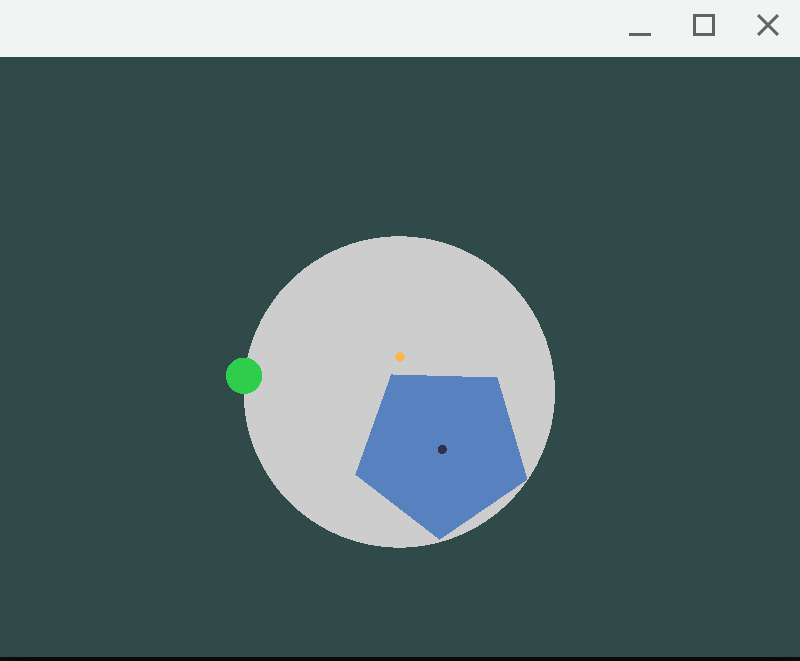
\includegraphics[height=5cm]{snaking.png}    \caption{In the snaking mode, the polygon stays close to the bottom of the boundary in the M-frame, and doesn't rotate.}
    \label{fig:snaking}
\end{figure}
However, for certain parameter sets, a trend toward counter-rotation is observed (see Figure: \ref{fig:down}), although the system appears very chaotic and the trend is only observed as an average across 500 trials. 
\begin{figure}
    \centering
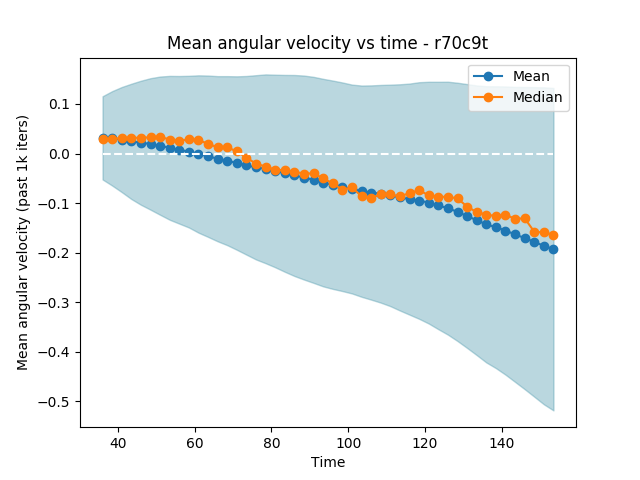
\includegraphics[height=6cm]{down.png}
   \caption{An octagon of radius 7 tends towards counterrotation. Visualized are the mean, median, and standard deviation range of the observed angular velocities versus times of 500 trials of an octagon of radius seven. }
    \label{fig:down}
\end{figure}
The trend appears to be related to the radius of the polygon, but in an as-of-yet undetermined manner. For instance, although snaking is universally seen for polygons of radius below 6, increasing the radius of the polygon beyond 7 can actually decrease the counter-rotation phenomenon observed above. 
\begin{figure}
    \centering
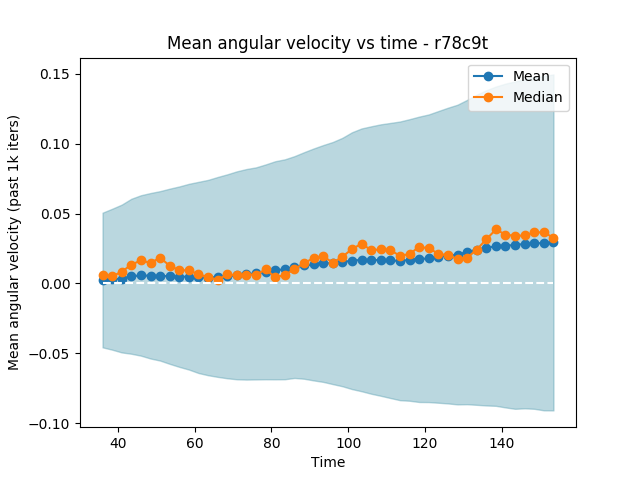
\includegraphics[height=6cm]{up.png}
  \caption{The same visualization as in Figure \ref{fig:down}, but the radius is increased to 7.8. Now the counter-rotation trend is lost. }
    \label{fig:up}
\end{figure}

\end{document}

